%%%%%%%%%%%%%%%%%%%%%%%%%%%%%%%%%%%%%%%%%
% University/School Laboratory Report
% LaTeX Template
% Version 1 (19/10/2019)
%
%%%%%%%%%%%%%%%%%%%%%%%%%%%%%%%%%%%%%%%%%

%----------------------------------------------------------------------------------------
%	PACKAGES AND DOCUMENT CONFIGURATIONS
%----------------------------------------------------------------------------------------

\documentclass{article}

\usepackage[version=3]{mhchem} % Package for chemical equation typesetting
\usepackage[inter-unit-product =\cdot]{siunitx} % Provides the \SI{}{} and \si{} command for typesetting SI units
\usepackage{graphicx} % Required for the inclusion of images
\usepackage{natbib} % Required to change bibliography style to APA
\usepackage{amsmath} % Required for some math elements 
\usepackage{breqn} %Required for dmath

\usepackage{graphicx} %Required for image

\setlength\parindent{0pt} % Removes all indentation from paragraphs

\renewcommand{\labelenumi}{\alph{enumi}.} % Make numbering in the enumerate environment by letter rather than number (e.g. section 6)


%\usepackage{times} % Uncomment to use the Times New Roman font

%----------------------------------------------------------------------------------------
%	DOCUMENT INFORMATION
%----------------------------------------------------------------------------------------

\title{Signal and sistems \\ Laboratory work - Inverted pendulum stabilization \\ COUAP-4109} % Title

\author{Josef \textsc{Sanda} \& Derin \textsc{Savran}} % Author name

\date{\today} % Date for the report

\begin{document}

\maketitle % Insert the title, author and date

\begin{center}
\begin{tabular}{l r}
Proposed by & Arben Cela % Instructor/supervisor
\end{tabular}
\end{center}
\begin{figure}[ht!]
    \centering
    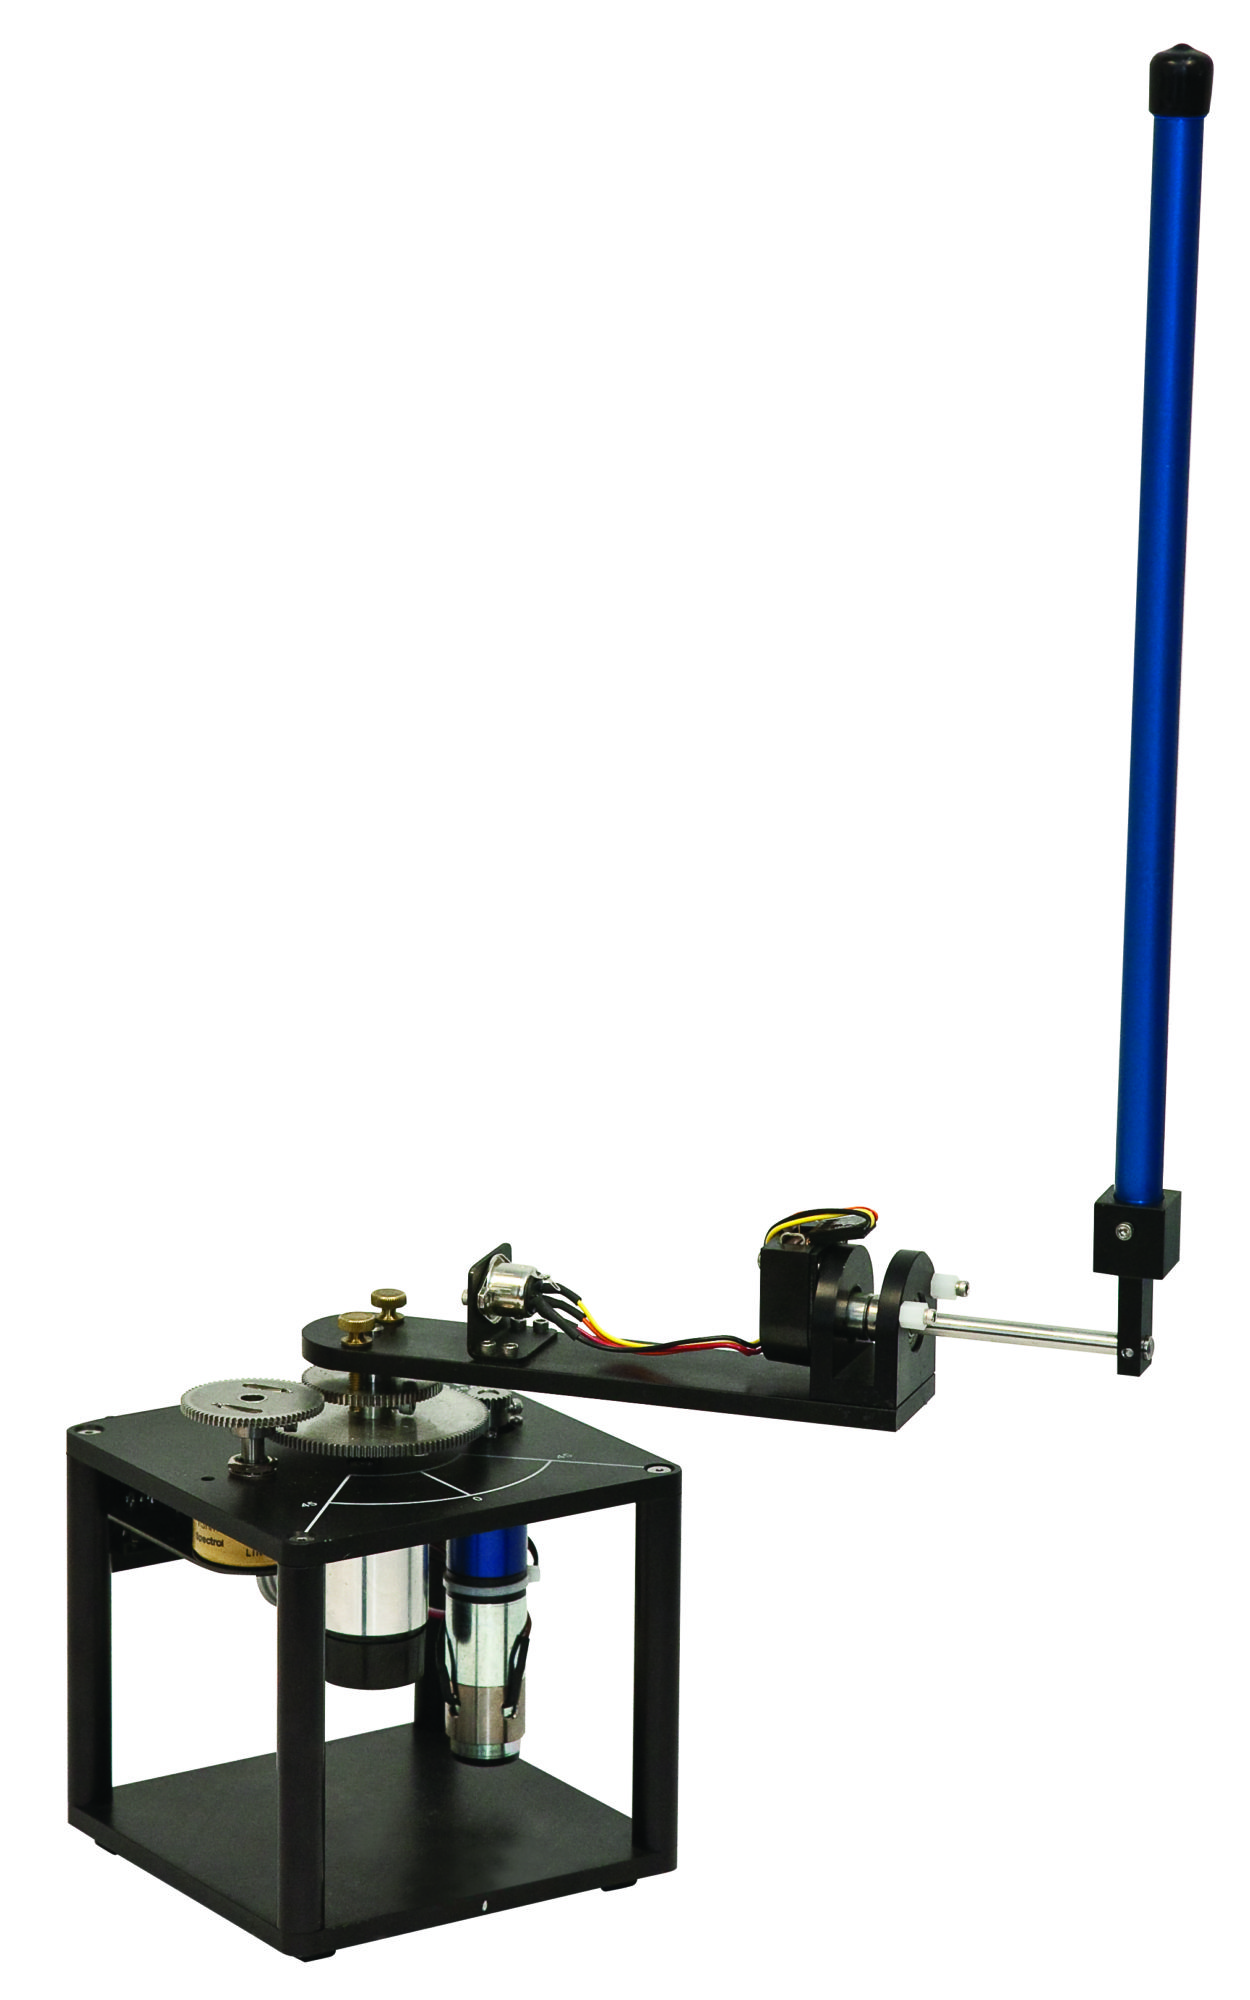
\includegraphics[scale=0.13]{img/rotary_inverted_pendulum.jpg}
    \caption{Laboratory module \label{fig:laboratory_module}}
\end{figure}

% If you wish to include an abstract, uncomment the lines below
% \begin{abstract}
% Abstract text
% \end{abstract}

\setlength{\parindent}{4em}
\setlength{\parskip}{1em}
\renewcommand{\baselinestretch}{2.0}

%----------------------------------------------------------------------------------------
%	SECTION 1
%----------------------------------------------------------------------------------------

\section{Incroduction}
% If you have more than one objective, uncomment the below:
%\begin{description}
%\item[First Objective] \hfill \\
%Objective 1 text
%\item[Second Objective] \hfill \\
%Objective 2 text
%\end{description}


\paragraph{}
The objective of this work is to stabilize the inverted pendulum in an upright position. For stabilization is used feedback controller based on the pole placement method. The pendulum consists of a driven arm. This arm rotates in the horizontal plane, and a pendulum attached to that arm is free to rotate in the vertical plane $[-\frac{\pi}{8}, +\frac{\pi}{8}]$. The arm has powered by the $\pm \si{10\volt}$ DC motor with constraints movement around. 
\paragraph{}
The system is exceptionally non-linear due to the gravitational forces that affect him. To realize the stabilization of this system, we have the possibility to use two sensors that measure with a satisfactory defect. The first sensor measures the position of the rod angle relative to the vertical position, and the second sensor measures the position of the arm motor angle. Both sensors have powered a voltage of $\pm \si{1,33\volt}$.
 
%----------------------------------------------------------------------------------------
%	SECTION 2
%----------------------------------------------------------------------------------------

\section{Model of a rotary pendulum}

The non-linear equation are given by 
\begin{dmath}\label{first_non_linear_equation_of_motion}
    \displaystyle {\ddot {\theta }}_{1}\left(J_{1zz}+m_{1}l_{1}^{2}+m_{2}L_{1}^{2}+(J_{2yy}+m_{2}l_{2}^{2})\sin ^{2}(\theta _{2})+J_{2xx}\cos ^{2}(\theta _{2})\right)+{\ddot {\theta }}_{2}m_{2}L_{1}l_{2}\cos(\theta _{2})-m_{2}L_{1}l_{2}\sin(\theta _{2}){\dot {\theta }}_{2}^{2}+{\dot {\theta }}_{1}{\dot {\theta }}_{2}\sin(2\theta _{2})(m_{2}l_{2}^{2}+J_{2yy}-J_{2xx})+b_{1}{\dot {\theta }}_{1}=\tau _{1}
\end{dmath}

and 

\begin{dmath}\label{second_non_linear_equation_of_motion}
    \displaystyle {\ddot {\theta }}_{1}m_{2}L_{1}l_{2}\cos(\theta _{2})+{\ddot {\theta }}_{2}(m_{2}l_{2}^{2}+J_{2zz})+1/2{\dot {\theta }}_{1}^{2}\sin(2\theta _{2})(-m_{2}l_{2}^{2}-J_{2yy}+J_{2xx})+b_{2}{\dot {\theta }}_{2}+gm_{2}l_{2}\sin(\theta _{2})=\tau _{2}
\end{dmath}


These equations are required by Broyden's method, which is the method for developing non-linear mathematical models like in Figure \ref{fig:model_of_inverted_pendulum} on page \pageref{fig:model_of_inverted_pendulum}.

\begin{figure}[ht!]
    \centering
    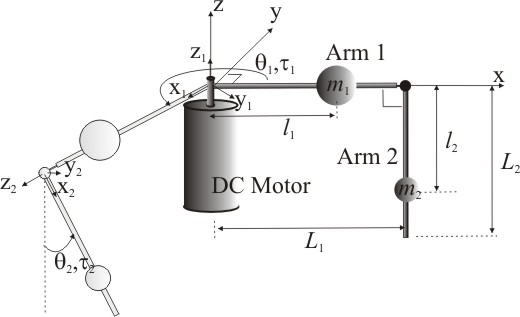
\includegraphics[scale=0.5]{img/Furuta_pendulum.jpg}
    \caption{Model of Inverted Pendulum \label{fig:model_of_inverted_pendulum}}
\end{figure}
%----------------------------------------------------------------------------------------
%	SECTION 3
%----------------------------------------------------------------------------------------

\section{Sample Calculation}

\begin{tabular}{ll}
Mass of magnesium metal & = \SI{8.59}{\gram} - \SI{7.28}{\gram}\\
& = \SI{1.31}{\gram}\\
Mass of magnesium oxide & = \SI{9.46}{\gram} - \SI{7.28}{\gram}\\
& = \SI{2.18}{\gram}\\
Mass of oxygen & = \SI{2.18}{\gram} - \SI{1.31}{\gram}\\
& = \SI{0.87}{\gram}
\end{tabular}

Because of this reaction, the required ratio is the atomic weight of magnesium: \SI{16.00}{\gram} of oxygen as experimental mass of Mg: experimental mass of oxygen or $\frac{x}{1.31}=\frac{16}{0.87}$ from which, $M_{\ce{Mg}} = 16.00 \times \frac{1.31}{0.87} = 24.1 = \SI{24}{\gram\per\mole}$ (to two significant figures).

%----------------------------------------------------------------------------------------
%	SECTION 4
%----------------------------------------------------------------------------------------

\section{Results and Conclusions}

The atomic weight of magnesium is concluded to be \SI{24}{\gram\per\mol}, as determined by the stoichiometry of its chemical combination with oxygen. This result is in agreement with the accepted value.

\begin{figure}[h]
\begin{center}

\includegraphics[width=0.65\textwidth]{placeholder} % Include the image placeholder.png
\caption{Figure caption.}
\end{center}
\end{figure}

%----------------------------------------------------------------------------------------
%	SECTION 5
%----------------------------------------------------------------------------------------

\section{Discussion of Experimental Uncertainty}

The accepted value (periodic table) is \SI{24.3}{\gram\per\mole} \cite{Smith:2012qr}. The percentage discrepancy between the accepted value and the result obtained here is 1.3\%. Because only a single measurement was made, it is not possible to calculate an estimated standard deviation.

The most obvious source of experimental uncertainty is the limited precision of the balance. Other potential sources of experimental uncertainty are: the reaction might not be complete; if not enough time was allowed for total oxidation, less than complete oxidation of the magnesium might have, in part, reacted with nitrogen in the air (incorrect reaction); the magnesium oxide might have absorbed water from the air, and thus weigh ``too much." Because the result obtained is close to the accepted value it is possible that some of these experimental uncertainties have fortuitously cancelled one another.

%----------------------------------------------------------------------------------------
%	SECTION 6
%----------------------------------------------------------------------------------------

\section{Answers to Definitions}

\begin{enumerate}
\begin{item}
The \emph{atomic weight of an element} is the relative weight of one of its atoms compared to C-12 with a weight of 12.0000000$\ldots$, hydrogen with a weight of 1.008, to oxygen with a weight of 16.00. Atomic weight is also the average weight of all the atoms of that element as they occur in nature.
\end{item}
\begin{item}
The \emph{units of atomic weight} are two-fold, with an identical numerical value. They are g/mole of atoms (or just g/mol) or amu/atom.
\end{item}
\begin{item}
\emph{Percentage discrepancy} between an accepted (literature) value and an experimental value is
\begin{equation*}
\frac{\mathrm{experimental\;result} - \mathrm{accepted\;result}}{\mathrm{accepted\;result}}
\end{equation*}
\end{item}
\end{enumerate}

%----------------------------------------------------------------------------------------
%	BIBLIOGRAPHY
%----------------------------------------------------------------------------------------

\bibliographystyle{apalike}

\bibliography{sample}

%----------------------------------------------------------------------------------------


\end{document}